\chapter{Design}\label{ch:design}

In this chapter we discuss the design of our system for managing timely dataflow
computations. It provides two main services which we discuss separately:
First, deployment and execution of submitted Timely programs, and secondly,
sharing of data streams between running timely dataflow computations.

\section{Overall Architecture}

Our system consists of multiple components which we briefly describe here:
A dataflow program submitted to run as part of the system is
called a \emph{query}. Following Timely's terminology, the execution of a query
is done by a group of \emph{worker} threads. Each worker manages the scheduling and
progress tracking of the operator in the dataflow graph. 

A query is executed by one or more \emph{executors}. Each executor selected to
execute a query will fetch and launch the query binary, ultimately spawning the
worker threads.

All these components are managed by a central process called the \emph{coordinator},
which stores and exposes the system state in the \emph{catalog}. The catalog includes
the list of the available executors, the running queries and what topics they
are processing.

In addition to managing query execution, the coordinator also provides services
for query composition: Queries can publish the results of their dataflow
computation as \emph{topics}, which in turn other queries can subscribe to.

\begin{figure}[p]
  \centering
    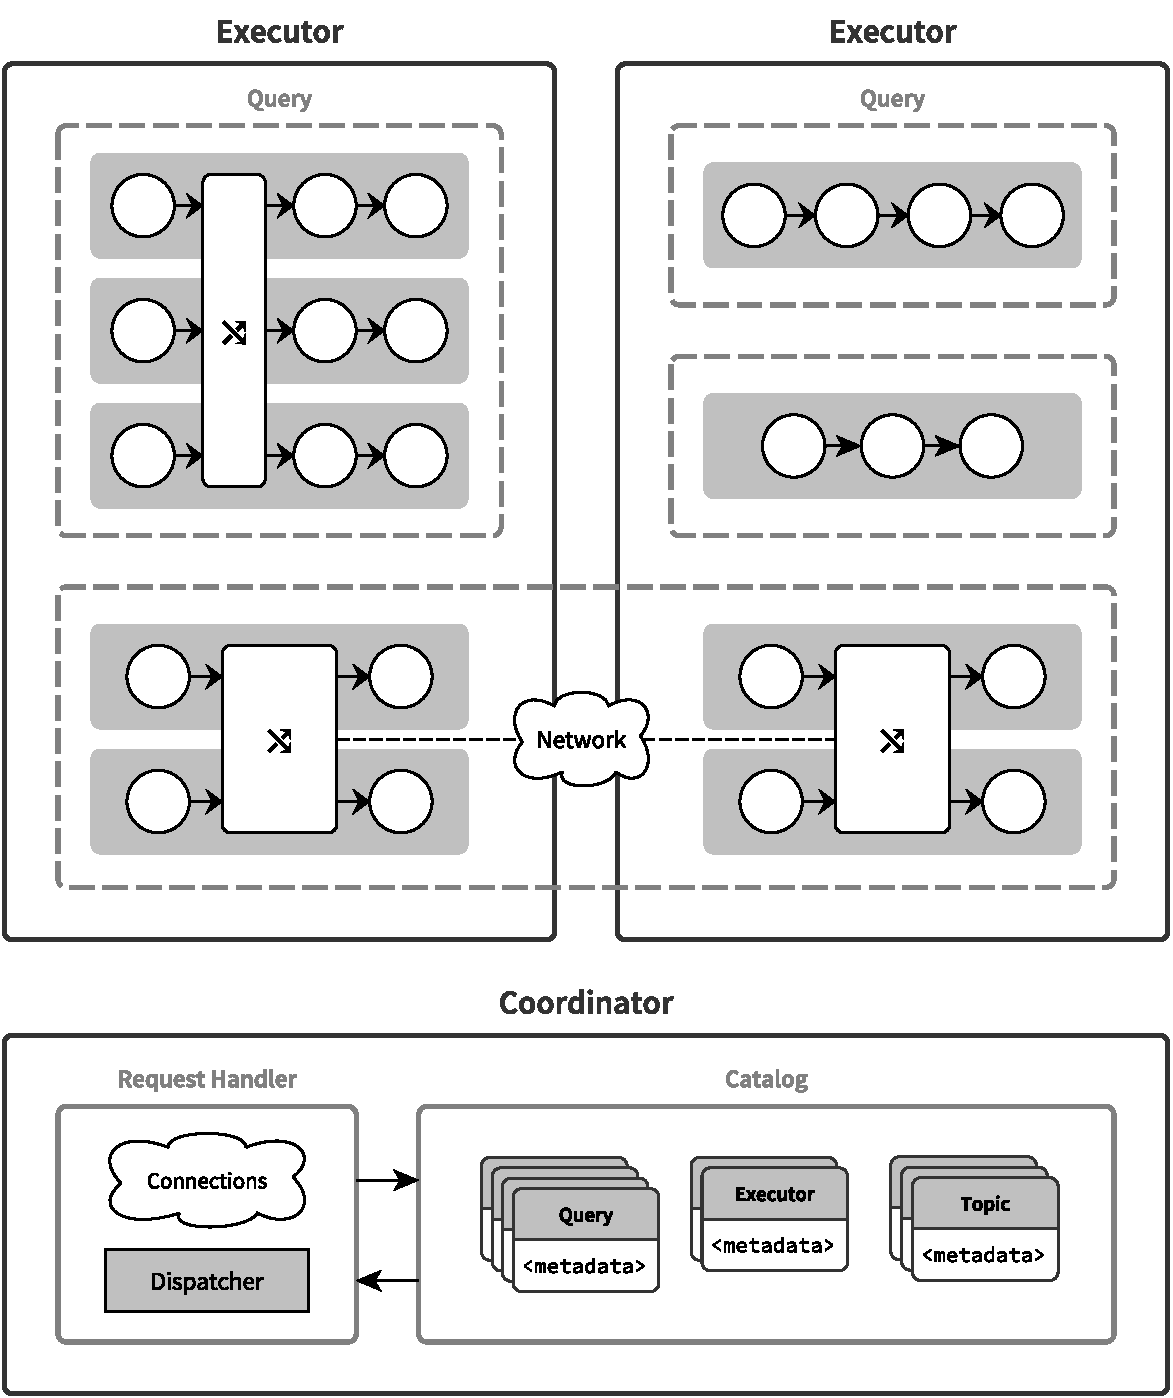
\includegraphics[width=1\textwidth]{figures/components}
  \caption[System architecture.]{ Queries (dashed boxes) consist of one or
  more worker threads (rounded grey boxes) driving the dataflow computation.
  A query might span over multiple executors, makeing use of the network for message exchanges
  between the workers of a query.\\
  The coordinator maintains a connection to every  executor and every query process.
  The state of the whole system is stored in the catalog.}
  \label{fig:components}
\end{figure}

\begin{table}
    \myfloatalign
  \begin{tabularx}{\textwidth}{>{\scshape}lX} \toprule
    \tableheadline{Component} & \tableheadline{Description} \\ \midrule
    Query & User-submitted Timely program running in the system.\\
    Worker & Thread belonging to a query, driving the computation of its local dataflow graph instance.  \\
    Executor & Process designated to host and spawn queries. \\
    Coordinator & Central process managing all the other components.\\
    Catalog & Data collection storing and exposing the system state at the coordinator.\\
    Topic & A named and typed representation of an exposed data stream.\\
    Publisher & Operator for exposing Timely streams by publishing them as a topic.\\
    Subscriber & Consumer of a stream emitted by a given topic.\\
    % submission
    % dataflow graph
    \bottomrule
  \end{tabularx}
  \caption{Terminology of the system.}  \label{tab:design-terminology}
\end{table}


\clearpage

\section{Queries}

A query is a Timely program managed and executed by our system. Like
standalone Timely Dataflow programs, queries are written in Rust and linked
against the Timely Dataflow library. The dataflow graph is constructed by connecting
Timely's operators (vertices) to stream objects (edges).

In standalone Timely applications, the user has to manually provide a configuration
for the worker threads. In our system, this information is partially generated by
the system, based on a user-provided template. Thus, we require that a query
registers its computational logic with our \lstinline{timely_query::execute} function,
instead of calling Time\-ly's initialization function directly.

This means that in order for a Timely Dataflow program to become a runnable
query in our the system, it needs to link against our \lstinline{timely_query} library.
This library not only performs the initialization of the Timely run-time, it also
provides additional functionality to interact with the coordinator, which we
describe below in section \fullref{sec:sharingstreams}.

Other than this, we do not want to impose any restrictions on what a query program
can do, it is free to execute arbitrary code.

\begin{lstlisting}[caption={[Example query.]Example query which prints out a stream of integers.}]
extern crate timely;
extern crate timely_query;

use timely::dataflow::Scope;
use timely::dataflow::operators::{Filter, Inspect, ToStream};

fn main() {
  timely_query::execute(|root, coordinator| {
    root.scoped::<u32, _, _>(|scope| {
      (0..100).to_stream(scope)
              .inspect(|x| println!("hello {:?}", x));
    });
  }).unwrap();
}
\end{lstlisting}

\section{Coordinator}

The coordinator is the central process of the system, managing all other
components. 
The coordinator provides an interface for users to submit new queries and
inspect the current state of the system. In order to receive commands and
report their internal state, every executor and query process maintains a
network connection to the coordinator.

Bookkeeping of the system is done by the coordinator in the catalog. The
catalog is a datastructure which contains all information about the available
executors, the running queries and their workers. This data is exposed to
queries through so called \emph{collection topics}, which we will describe
below. This allows queries to introspect the system state using Timely operators.

\subsection{Submission}

A query is submitted to the coordinator as a binary executable. Compilation
is done externally to allow the use of third-party libraries. A submission
consists of the location of the query binary, as well as the runtime
configuration for the workers. The runtime configuration specifies the amount
and distribution of the worker threads which will drive the query.

Optionally, a human-readable description of the query,
as well as the command-line arguments to be passed to the executable can be
provided.

When handling a new query submission request, the coordinator will assign a
unique identifier to the incoming query, and then select a
matching number of executors for the query to be spawned on. The selection
of executors is based on the runtime configuration provided by the submission
request.

The coordinator plays an important role when spawning new queries. After
issuing query spawn requests to the executors, it waits for all query processes
to register themselves at the coordinator before they begin their computation.
Only then the query is considered active and the submission request
is reported to be completed.

\begin{figure}[htb]
  \centering
    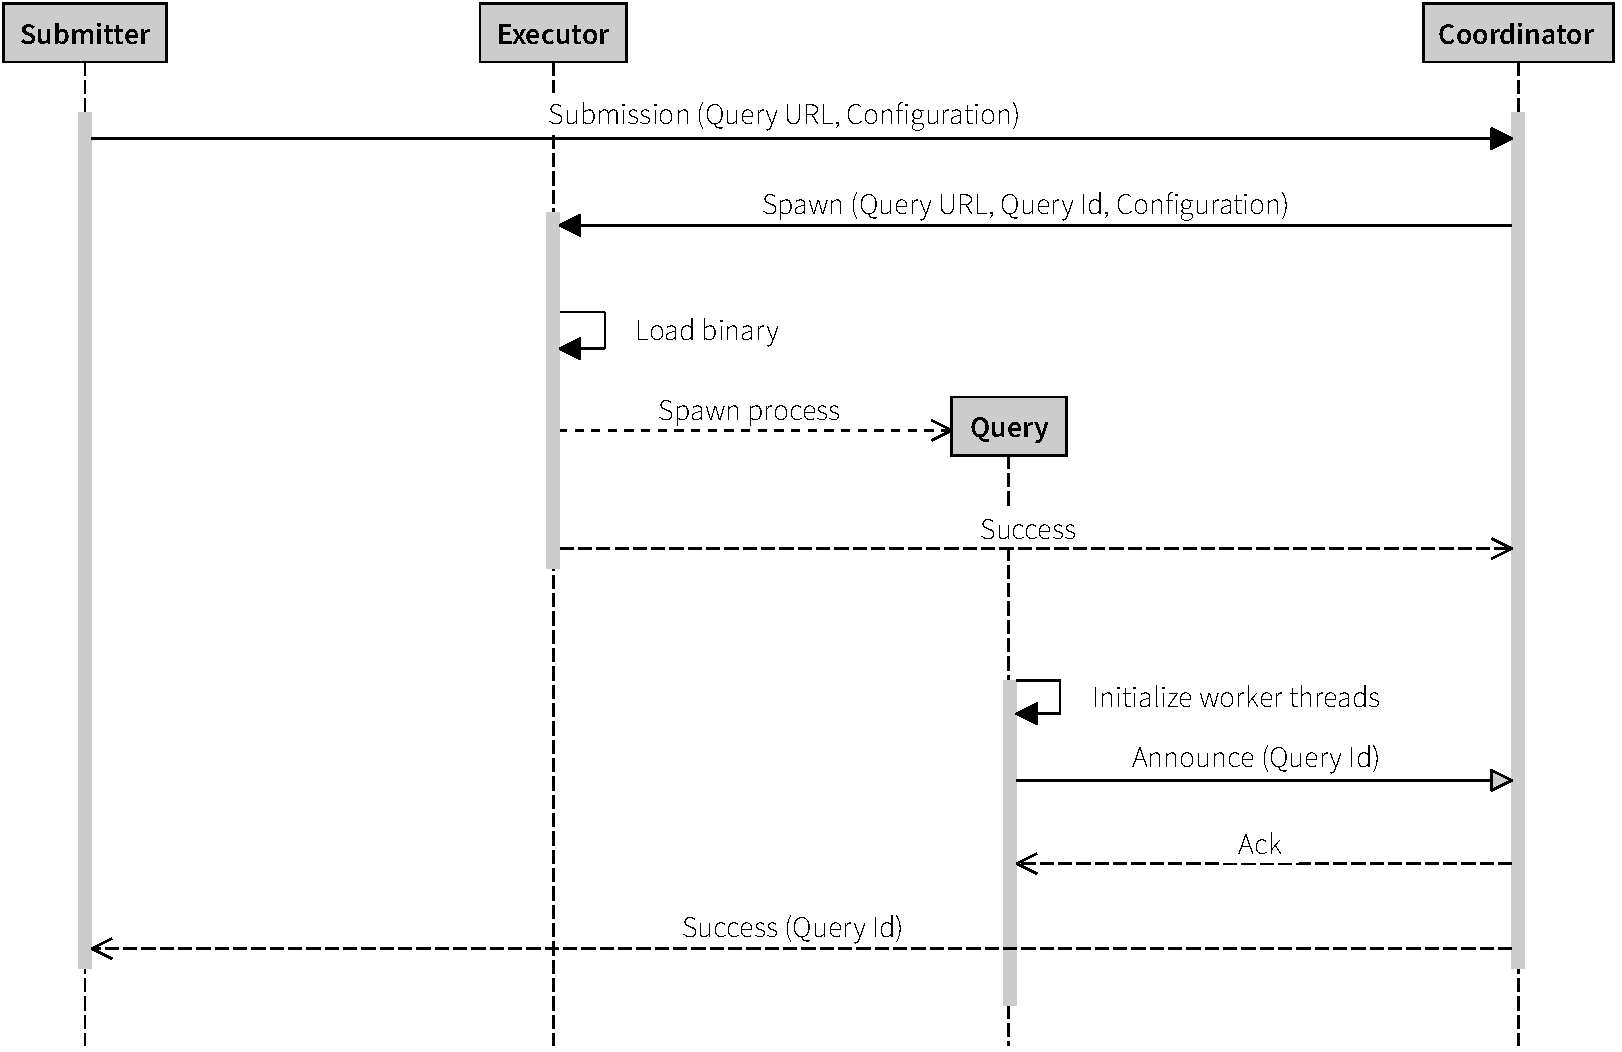
\includegraphics[width=1\textwidth]{figures/spawn_singleprocess}
  \caption[Query submission with single process.]{Submission of a query on a single executor.
  Only once the spawned query announces itself at the coordinator is it considered running.}
  \label{fig:subsingle}
\end{figure}

\section{Executors}

The spawning and direct supervision of query processes is not done by the
coordinator itself, but is offloaded to designated processes called executors.
This choice allows for more flexibility regarding query execution and the
management of available resources. Since executors can be dynamically added
to the system, and with some limitations also be removed again, they provide
a way for adding new machines to the cluster running our system. The catalog
maintains the pool of available executors which are participating in the system.

As a timely program can span over multiple machines, a query might span
over multiple executors. The placement of a query on the available executors
is performed by the coordinator, based on the users request.
We currently implement a naive approach to query placement, where the executors
are chosen randomly if the user does not manually specify a placement. A more
sophisticated scheduling, which for example could include load balancing,
has to be investigated.

Another feature of executors is that they define how queries and their
worker threads are supposed to be executed. When an executor joins
the system by introducing itself to the coordinator, the executor also informs
the coordinator about the execution format it supports. In the current
implementation, executors only support the execution of queries in the form of
native operating system executables.

When spawning such an executable, the newly spawned query process
performs the worker initialization on behalf of the executor. 
The executor supplies the newly created process with the information
it needs in order to participate in the system. This includes the query's own identifier,
the address of the coordinator, the addresses of any peer processes belonging to the 
same query, and the number of worker threads to spawn inside this process.

Executors are also responsible for fetching any query binaries they are supposed
to spawn. When submitting a new query, the submitter has to provide coordinator
with the location of the binary. This location is forwarded to participating executors,
which will use it to load the query binary. 

Since executors serve as a provider for computational resources such as machines,
there is typically a one-to-one mapping between executors and the machines they
are running on. This however is not a requirement of the system, the deployment of
executors is left to the user. Similarly, the user is free spawn multiple
processes belonging to the same query on the same executor if they wish to do so.

Since operating system processes can outlive their parent process, executors can
be removed from the system while the queries spawned by the executor are still
running. In this case, the coordinator removes the terminating executor from
the pool, disallowing any future queries to be hosted on the removed executor.

\paragraph{Future Considerations}

The current implementation of executors which run queries in their own separate
process is not the only possible implementation choice.
Alternative implementations could for example host multiple queries
within the same process, by dynamically loading the query's code into an already
running process and run it on a preemptive operating system thread. This would allow queries
the interchange of objects without the need for data serialization. Given
the implementation of Timely's operator scheduling, cooperative scheduling
of multiple worker threads within a single operating system thread could also
be implemented for certain queries where its input is managed by the system.


\section{Sharing Data Streams} \label{sec:sharingstreams}

Dataflow programs typically work on streams from external sources. As the same
data source might be of interest for different dataflow computations, it seems
appropriate to manage data streams in our system as well. Furthermore,
input streams might not only come from external sources: A dataflow computation
might produce an intermediate or final output stream which could be of interest
for other queries. These assumptions motivate us to extend our system with a
mechanism to allow queries to expose their data streams for consumption by other
queries.

We implement this in the form of a topic-based publish/subscribe system:
Using the \emph{publish} operator, a query can expose one of its streams
(an edge in the dataflow graph) to other queries, which in turn then \emph{subscribe}
to it. The list of all published topics is stored at in the catalog.

The reason for choosing a topic-based publish/subscribe system over a
content- or type-based one is dictated by the fact that Rust allows for little
type introspection. In addition, having users explicitly publish and name
exposed streams helps to differentiate between streams with the same datatype
but different semantics.

For providing access to external inputs, we require that a designated query
translates these external inputs into Timely streams and publishes the result as
a topic. We prefer this manual approach over providing our own adapters, as there
already exists a rich collection of Timely-aware code which performs this
translation of external input to Timely streams.

\subsection{Topics}

A topic has the following properties, which are all stored in the catalog
and can be accessed by other queries.
\begin{description}
\item [Identifier] A unique identifier for the topic instance.
\item [Name] When publishing a stream, the publisher has to assign a name to it.
Queries use this name to refer to topics they want to subscribe to. There might
be only one topic with a certain name at a time, however names can be reused if
topics are unpublished.
\item [Schema] A descriptor of the data type of the stream published in this
topic. Timely's streams are typed channels, therefore so are topics.
\item [Address] An address to which the subscribers connect in order to received
the contents of the published stream.
\end{description}

While every publication and subscription request is disclosed to the coordinator
and the catalog contains a list of all existing topics, the
actual exchange of data happens directly between queries. When a query subscribes
to a topic, it receives the address of the topic's publisher from the coordinator
and directly connects to it.

\subsection{Stream Publisher}

A stream publisher is a Timely operator which exposes a Timely stream as a topic. When
creating it, the query author has to assign a name for the topic under which the
input stream will be published. As with all other Timely operators, the publisher
operator is instantiated on all worker threads. However, the user can choose
whether all worker streams are merged into a single topic before publishing, or
if each worker publishes its own topic. The latter option implicitly exposes
the data sharding strategy of the publishing query, allowing the workers of
the subscribing query to exploit this partition scheme.

\subsubsection{Collection Publisher}

Our publishers are not buffered, meaning subscribers will
not receive any data which was produced before they subscribed to a certain
topic. This is the same as in many other publish/subscribe systems, where
synchronization between publishers and subscribers is decoupled as well. \cite{pubsub}

However, in streams where the contents of the stream describes changes of a certain
state, it is essential for stream consumers to know the state of the source at
the beginning of the stream in order to make sense out of it. The motivating
example here is the catalog, which is supposed to expose the current system state to
new participants.

For this reason, we introduce a second kind of publisher which publishes
\emph{collections} instead of streams. A collection in our model is a typed, unordered
multiset maintained by the publisher, possibly representing state it would
like to share with subscribers.

Upon creation, a collection publisher contains an empty collection.
When the publishing query mutates the collection by adding or removing elements,
these changes are propagated to the subscribers. When new subscribers connect
to this publisher, the publisher will provide them with a list of all currently
contained elements. This way, all subscribers eventually maintain the same view
of the data collection.

From the subscribers point of view, a topic published by a collection publisher
is not inherently different from a normal topic: After subscribing, it will
observe a continuous stream of data. The difference is in the data type of the
stream, it will be of tuples of the format $(\texttt{Data}, \delta)$, where
\texttt{Data} is an element that can be stored in the multiset and $\delta$ 
is a signed integer denoting the amount of elements that have been added or removed from the set.
This format is compatible with the notion of collections in Differential Dataflow \cite{differential},
allowing subscribing queries to further process the collection in a convenient
manner. Note however that our collections are not versioned, we
do not append timestamps to the update messages.

\subsection{Subscriber}

In order to subscribe to a topic, the subscribing query has to provide the name
of the topic it is interested in. This involves a name lookup which can optionally
be blocking: If a requested topic does not yet exist, the coordinator will add
the subscriber to a wait list. Once a corresponding topic is published under that
name, the coordinator will inform the subscriber about this topic. 

The subscribing query is free to subscribe to multiple topics. It the query's
responsibility to merge and feed the data streams into the dataflow graph.

\subsection{Comparison with Timely's Capture \& Replay}

The Timely library provides special capture and replay operators which also serve the
purpose of sharing data between queries. With the capture operator, all timestamp,
data and event records are collected in one dataflow computation,
and can then be replayed in another one.

The capture/replay operators will record and replay the whole stream from beginning
to end, requiring the capture operator to either buffer its incoming data or
wait for the replaying query to connect to it. 
In our system, we opted for a more dynamic approach, where
producing queries are allowed to discard data if there are no consumers.

It is the responsibility of the user to provide a communication channel between
capture and  replay operators. Adapters exist for Rust's thread-safe FIFO queues,
single-threaded queues, file handles and sockets.

